\documentclass{article}
\usepackage[utf8]{inputenc}
\documentclass[12pt]{article}
%\usepackage[left=3cm, right=2.5cm, top=2.5cm, bottom=2.5cm]{geometry}e}
\usepackage[utf8]{inputenc}
\usepackage[spanish,english]{babel}
\usepackage{apacite}
\usepackage[round]{natbib}
\usepackage{hyperref}
\usepackage{float}
\usepackage{svg}
\usepackage[margin = 1in, top=2cm]{geometry}% Margins
\setlength{\parindent}{2em}
\setlength{\parskip}{0.2em}
\usepackage{setspace} % Setting the spacing between lines
\usepackage{amsthm, amsmath, amsfonts, mathtools, amssymb, bm} % Math packages 
\usepackage{svg}
\usepackage{graphicx}
\usepackage{pgfplots}
\usepackage{epstopdf}
\usepackage{subfig} % Manipulation and reference of small or sub figures and tables
\usepackage{hyperref} % To create hyperlinks within the document
\spacing{1.15}
\usepackage{appendix}
\usepackage{xcolor}
\usepackage{cancel}
\usepackage{enumerate}
\usepackage[shortlabels]{enumitem}


\usepackage[round]{natbib}
%\bibliographystyle{plainnat}
\bibliographystyle{apacite}


\newtheorem{defin}{Definition.}
\newtheorem{teo}{Theorem. }
\newtheorem{lema}{Lemma. }
\newtheorem{coro}{Corolary. }
\newtheorem{prop}{Proposition. }
\theoremstyle{definition}
\newtheorem{examp}{Example. }
\newtheorem{problem}{Problem}
\newtheorem{subproblem}{}[problem]
% \numberwithin{problem}{subsection} 

\newcommand{\card}{\operatorname{card}}
\newcommand{\qiq}{\qquad \implies \qquad}
\newcommand{\qiffq}{\qquad \iff \qquad}
\newcommand{\qaq}{\qquad \textbf{and} \qquad}
\newcommand{\qoq}{\qquad \textbf{or} \qquad}
\newcommand{\settf}{\text{ \emph{:} }}
\newcommand{\chbox}{\makebox[0pt][l]{$\square$}\raisebox{.15ex}{\hspace{.9em}}}
\newcommand{\cchbox}{\makebox[0pt][l]{$\square$}\raisebox{.15ex}{\hspace{0.1em}$\checkmark$}}

\title{Problem Set 3}
\author{Mitchell Valdés-Bobes}
\date{September 23, 2020}

\begin{document}

\maketitle
\begin{problem}
Consider the following overlapping generations problem. In each period $t=1,2,3, \ldots$ a new
generation of 2 period lived households are born. Each generation has a unitary mass. There
is a unit measure of initial old who are endowed with $\bar{M}>0$ units of fiat money. Each
generation is endowed with $w_{1}$ in youth and $w_{2}$ in old age of non-storable consumption goods
where $w_{1}>w_{2}$. There is no commitment technology to enforce trades. The utility function
of a household of generation $t \geq 1$ is
$$
U\left(c_{t}^{t}, c_{t+1}^{t}\right)=\ln \left(c_{t}^{t}\right)+\ln \left(c_{t+1}^{t}\right)
$$
where $\left(c_{i}^{t}, c_{i+1}^{t}\right)$ is consumption of a household of generation $t$ in youth (i.e. in period $t$ ) and
old age (i.e in period $t+1$ ). The preferences of the initial old are given by $U\left(c_{1}^{0}\right)=\ln \left(c_{1}^{0}\right)$
where $c_{1}^{0}$ is consumption by a household of the initial old.
\end{subproblem}
\begin{subproblem}
 State and solve the planner’s problem.
\end{subproblem}

\begin{proof}[Answer]
The planner maximises consumption for all agents that alive in each period, subject to the resource feasibility constraint (FC). The model is the following

\begin{align}
\max_{(c_t^{t-1}, c_t^t) \in \mathbb{R}^2_+}& \quad \sum_{t=1}^\infty \ln c_t^t + \ln c_t^{t-1}\\
\text{subject to} &\quad   c_t^{t-1}, c_t^t \leq w_1 + w_2 \quad \forall t\geq 1\tag{FC}
\end{align}

Since the objective function is increasing in both arguments, then we know that at the optimum (FC) will bind, therefore

\begin{equation}\label{bindingplaner}
c_t^{t-1}, c_t^t = w_1 + w_2  \qiq c_t = w_1 + w_2 - c^{t-1}_t \qquad \forall t\geq 0
\end{equation}

Now we only have to choose $c^t_{t-1}$ that maximizes the objective function:


\begin{align}
    \ln (w_1 + w_2 - c^{t-1}_t) + \ln c_t^{t-1}
\end{align}


The problem have the following set of First Order Conditions:
\begin{equation}\label{planer_ct1}
\text{FOC}_{t}: \quad -\frac{1}{w_1 + w_2 - c^{t-1}_t} + \frac{1}{c^{t-1}_t} = 0 \qiq \boxed{c_t^{t-1} = \frac{w_1+w_2}{2}} \quad \forall t\geq 1    
\end{equation}
Plugging \eqref{planer_ct1} in \eqref{bindingplaner} we get:
\begin{equation}{\label{planer_ct}}
\boxed{c_t^{t} = \frac{w_1+w_2}{2}}    
\end{equation}

And since the objective function is concave, we know that this is the solution for the maximization problem.

\end{proof}


\begin{subproblem}
State the representative household’s problem in period $t\geq0$. Try to write the budget constraints in real terms.
\end{subproblem}

\begin{proof}[Answer]
The initial old solve their maximization problem in $t=1$ subject to their budget constraint:

\begin{align}\label{initalold}
\max_{c^1_0\geq 0}&\quad \ln c^0_1  \\
\text{subject to} & \quad  c^0_1\leq \frac{\bar{M}}{p_1}+w_2\tag{BC}
\end{align}

The following generation maximize their consumption subject to their budget constraints:


\begin{align}\label{generalproblem}
\max_{(c^t_t,c^t_{t+1}, M_{t+1}^t)\in \mathbb{R}_+^3 }&\quad \ln c^t_t + \ln c^t_{t+1} \\
\text{subject to} & \quad   c^t_t +  \frac{M_{t+1}^t}{p_t}\leq w_1 \tag{$\text{BC}_{t}$}\\ 
& \quad c^t_{t+1} \leq w_2 + \frac{M_{t+1}^t}{p_2} \tag{$\text{BC}_{t+1}$}
\end{align}


\end{proof}

\begin{subroblem}
Define and solve for an autarkic equilibrium, assuming that it exists.
\end{problem}

\begin{proof}
The equilibrium in autarky is a set of allocations $\{c_t^{t-1}, c_t^t, M_t^{t-1}\}_{t=1}^\infty$ and a set of prices $\{p_t\}_{t=1}^\infty$ such that the market for money clears
\begin{equation}
M_t = \bar{M} \qquad \forall t \geq 1
\end{equation}

the market for goods clears
\begin{equation}
Nc_t^{t-1} + Nc_t^t  = N w_1 + N w_2 \qquad \forall t \geq 1
\end{equation}

And agents optimize, since there is no trade in autarchy nor any technology to store good, then agents consume all their endowment in each period:
\begin{align*}
    c_t^{t-1} = w_1\\c_t^t = w_2
\end{align}

Then the only sequence of prices that will support this equilibrium is when the first generation does not value money therefore:

$$\frac{1}{p_t}=0 \qquad \forall t\geq 1$$

\end{proof}

\begin{subproblem}
Define and solve for a competitive equilibrium assuming valued money but with $w_2 = 0$.
\end{subproblem}

\begin{proof}[Answer]
Remember that the initial old solve their maximization problem in $t=1$ subject to their budget constraint (problem in \eqref{initalold}):

since the utility function is increasing in consumption the initial old will consume all their endowment and the worth of the fiat money in consumption therefore:

\begin{equation}
c^0_1 = \frac{\bar{M}}{p_1}+w_2 \quad \text{if } w_2 = 0 \qiq \boxed{c^0_1 = \frac{\bar{M}}{p_1}}
\end{equation}

To solve the problem of the following generations we can collapse both budget constraints, make them binding and make $w_2=0$ to get the simplified problem :

\begin{align}\label{generalproblem}
\max_{(c^t_t,c^t_{t+1})\in \mathbb{R}_+^2 }&\quad \ln c^t_t + \ln c^t_{t+1} \\
\text{subject to} & \quad   \frac{p_t}{ p_{t+1}}(w_1 - c^t_t)= c^t_{t+1} \tag{BC}
\end{align}
Plugging the budget constraint in to the objective function we get:
\begin{align}\label{simprob}
\max_{c^t_t\in \mathbb{R}_+^2 }&\quad \ln c^t_t + \ln \left(\frac{p_t}{ p_{t+1}}(w_1 - c^t_t) \right)
\end{align}

The FOC of this problem give us:

\begin{equation}
\frac{1}{c_t}-\frac{1}{w_1-c_t} \qiq c_t = \frac{w_1}{2}\label{ctw20}
\end{equation}

Plugin \eqref{ctw20} in the budget constraint of \eqref{simprob} we obtain:

\begin{equation}\label{ct1w20}
   c^t_{t+1} = \frac{w_1 p_t}{2 p_{t+1}}
\end{equation}

To obtain the allocation of fiat money money, plug in \eqref{ctw20} in to the budget constraint for time $t$ in \eqref{generalproblem}:

\begin{equation}\label{Mw20}
\frac{w_1}{2} +  \frac{M_{t+1}^t}{p_t} = w_1 \qiq M^t_{t+1} = \frac{p_t w_1}{2}
\end{equation}

The \textbf{equilibrium} is a set of allocations $\{c_t^{t-1}, c_t^t, M_t^{t-1}\}_{t=1}^\infty$ and a set of prices $\{p_t\}_{t=1}^\infty$ such that the market for money clears
\begin{equation}
M_t = \bar{M} \qquad \forall t \geq 1
\end{equation}

the market for goods clears
\begin{equation}
Nc_t^{t-1} + Nc_t^t  = N w_1 + N w_2 \qquad \forall t \geq 1
\end{equation}

And agents optimize, according to \eqref{ctw20}, \eqref{ct1w20} and \eqref{Mw20}. For the optimality conditions and the market clearing to to hold simultaneously we need:

$$p_t = p_{t+1} =\bar{p} \qiq \bar{p}= \frac{2 \bar{M}}{w_1}$$

\end{proof}
\newpage
\begin{subproblem}
Compare the solutions to the planners problem, the autarky equilibrium and the stationary monetary competitive equilibrium with valued money, all with $w_2 = 0$
\end{subproblem}

\begin{proof}[Answer]

For the social planner problem we had the following solution:
$$c_{1}^{0}= \frac{w_1}{2} \qquad c_{t}^{t} = \frac{w_1}{2}  \qquad c_{t+1}^{t}= \frac{w_1}{2}$$
In autharchy we have:
$$c_{1}^{0}=0  \qquad c_{t}^{t} =w_1   \qquad c_{t+1}^{t}= 0$$
And in the monetary equilibrium:
$$c_{1}^{0}= \frac{w_1}{2} \qquad c_{t}^{t} = \frac{w_1}{2}  \qquad c_{t+1}^{t}= \frac{w_1}{2}$$

Clearly in autarchy all agents will get $-\infty$ utility since they have no means to transfer some of their consumption from period $t$ to period $t+1$.

When a social planner is allocating consumption he cares equally about all agents, therefore the agents are guaranteed half of their endowment from period $t$ in period $t+1$. The interesting part is that this``welfare maximizing'' allocation can also be achieved in a decentralized manner when the agents value the fiat money.

\end{proof}

\begin{subproblem}
What happens to consumption, money demand and prices in a competitive equilibrium
with valued money if the initial money supply is halved, i.e. $\bar{M}^{\prime}=\frac{M}{2}$. Keep the
assumption that $w_{2}=0$
\end{subproblem}

\begin{proof}[Answer]
We can see from solution, that the money supply does not affect the equilibrium allocation, therefore if we will have the same equilibrium consumption for $M'$ that we had for $M$.

On the other hand money demand and prices will go down in half:

$$
M_t' =  \bar{M}' = \frac{\bar{M}}{2} = \frac{M_t}{2} \qaq p_t' = \frac{2\bar{M}}{w_1} = \frac{2\bar{M}/2}{w_1} = \frac{p_t}{2}
$$

\end{proof}
\newpage
\begin{problem}
Plot the trade offer curves for the following utility functions where the endowment is $\left(w_{1}, w_{2}\right)$
for goods $1$ and $2,$ respectively.
\end{problem}

\begin{subproblem}
$U=10 x_{1}-4 x_{1}^{2}+4 x_{2}-x_{2}^{2},\left(w_{1}, w_{2}\right)=(0,2)$
\end{subproblem}

\begin{figure}[h]
    \centering
    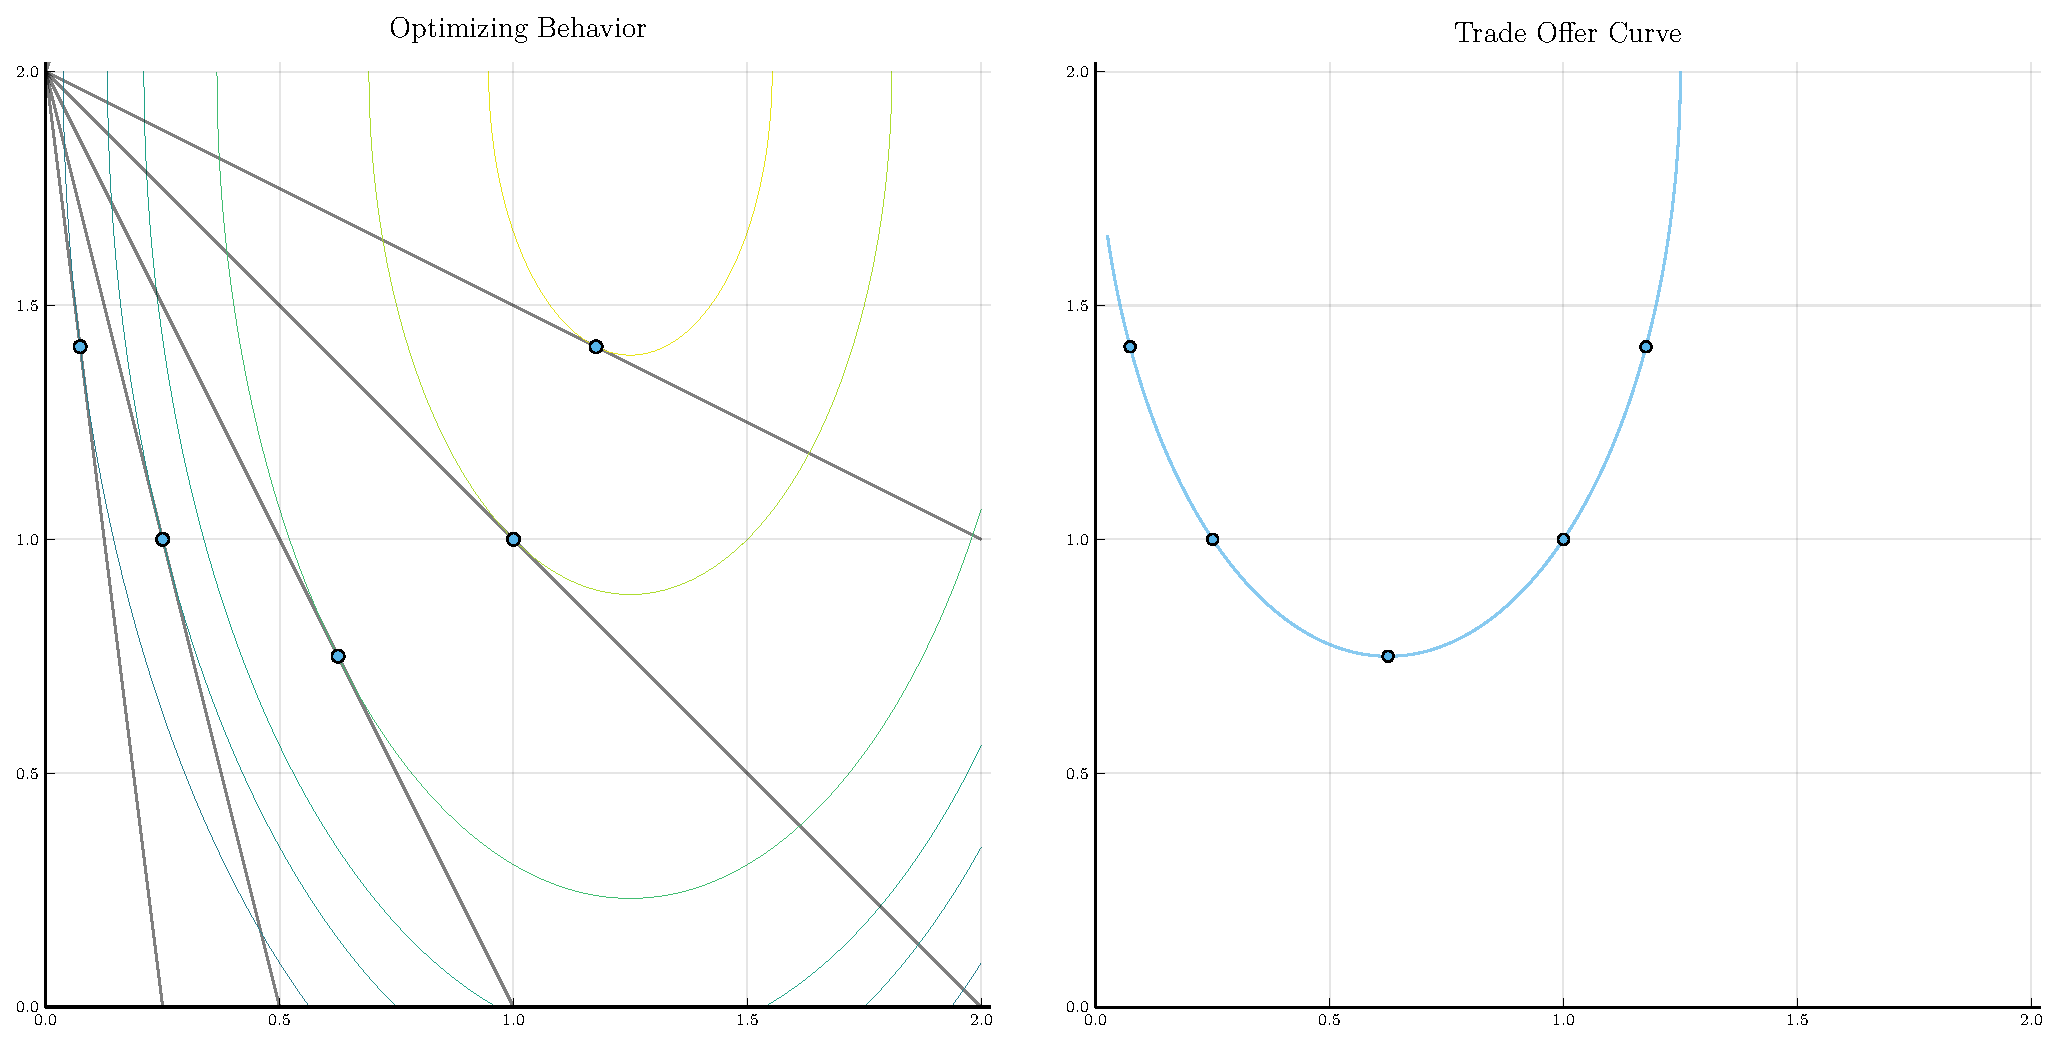
\includegraphics[width=1\linewidth]{Problem_Set_3_files/offer1.pdf}
    \label{fig:ex2_2}
\end{figure}

\newpage
\begin{subproblem}
$U=\min\left\{2 x_{1}+x_{2}, x_{1}+2 x_{2}\right\},\left(w_{1}, w_{2}\right)=(1,0)$
\end{subproblem}

\begin{figure}[h]
    \centering
    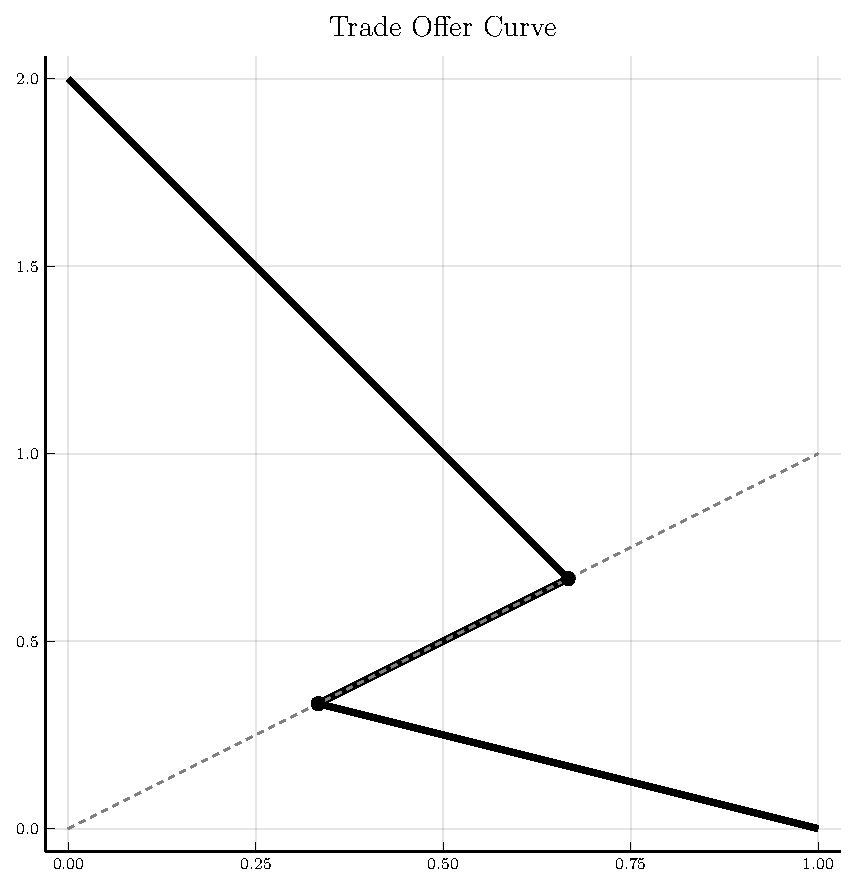
\includegraphics[width=.6\linewidth]{Problem_Set_3_files/offer2.pdf}
    \label{fig:ex2_2}
\end{figure}
\newpage
\begin{subproblem}
$U=\min \left\{2 x_{1}+x_{2}, x_{1}+2 x_{2}\right\},\left(w_{1}, w_{2}\right)=(1,10)$
\end{subproblem}

\begin{figure}[h]
    \centering
    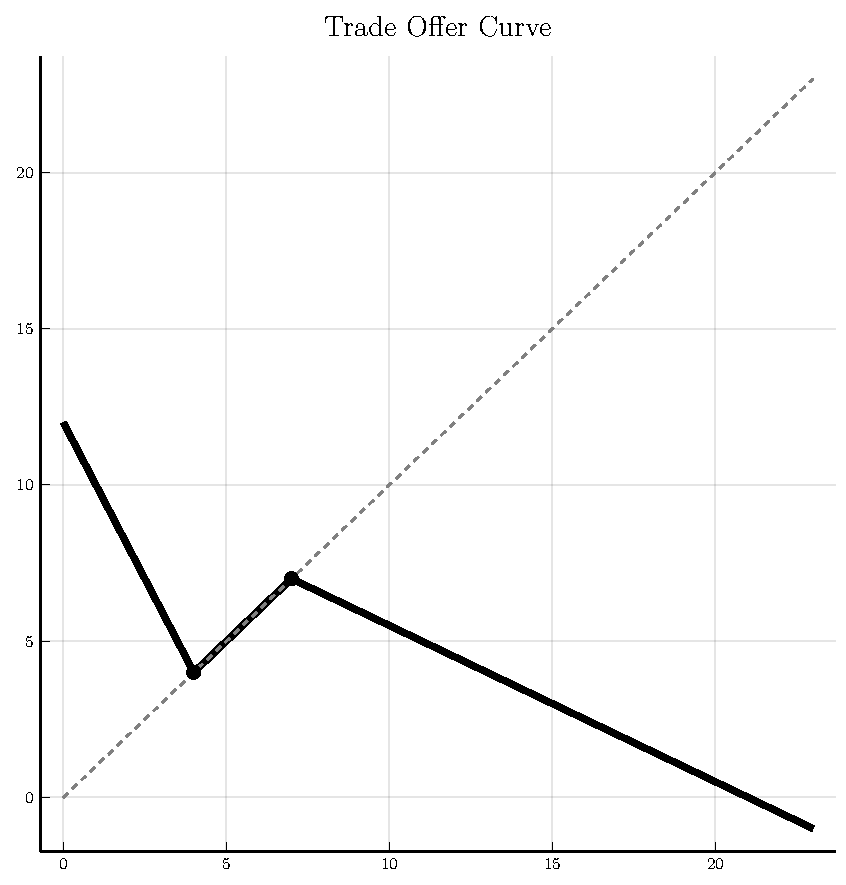
\includegraphics[width=.6\linewidth]{Problem_Set_3_files/offer3.pdf}
    \label{fig:ex2_2}
\end{figure}


\end{document}